% Template for Cogsci submission with R Markdown

% Stuff changed from original Markdown PLOS Template
\documentclass[10pt, letterpaper]{article}

\usepackage{cogsci}


\title{TODO}


\author{{\large \bf Veronica Boyce (vboyce@stanford.edu)} \\ Department of Psychology, \\Stanford University \And {\large \bf Ben (TODO email) } Department of Psychology, \\Stanford University \AND {\large \bf Alvin (TODO email)} \\ TODO affiliation, Stanford University \And {\large \bf Michael C. Frank (mcfrank@stanford.edu)} \\ Department of Psychology, \\ Stanford University}


\begin{document}

\maketitle

\begin{abstract}
TODO abstract

\textbf{Keywords:}
TODO keywords
\end{abstract}

\section{Introduction}\label{introduction}

Conversation pacts and partner specificity are often studied by looking
at how they are constructed; an additional perspective comes from how
opaque or interpretable they are to outsiders who weren't part of the
pact

By measuring opaqueness in different conditions related to how the pacts
were formed or what the language looks like, can get another perspective
on the process of pact formation

An empirical test of partner - specificity

Prior work to cover Summary of ref games \& claims around them
(\textbf{hawkins2020b?}) (\textbf{clark1986?}) etc

The side-participant / overhearer etc literature
(\textbf{wilkes-gibbs1992?}), \& lit search for more

Judy's work Visual resemblance and interaction history jointly constrain
pictorial meaning (\textbf{hawkinsb?})

possible could also mention other times when naive comprehender has been
used to better understand iteractive dialogues?

``Why use models'' -- can frame opaqueness as semantic distance between
utterance and referent -- models are an explicit test of this! ``Naive
comprehender'' / ``matcher''

\subsection{ALvin gets to write computational intro
here}\label{alvin-gets-to-write-computational-intro-here}

Do we also want to motivate this from a computational angle?
(i.e.~trying to add pragmatics to models) TODO not me

\subsection{back to Veronica}\label{back-to-veronica}

Key question: What properties of conversational pacts and the process of
their formation make them more or less easy for an outsider to
understand?

We use both human experiments and models to assess when and why
expressions are opaque or understandable to outside observers.

\section{Task Setup}\label{task-setup}

\subsection{Materials}\label{materials}

We draw on the corpus of reference game transcripts and results from
(\textbf{boyce2024?}). There were all 6 round iterated reference games
using the same 12 target images, but varied in how large the groups were
(2-6 participants per group) and how ``thick'' the communication channel
between group members was. For our human experiments, we sample
different subsets of this corpus in different experiments. We use the
entire corpus for our computational modelling component. TODO discussion
of (\textbf{boyce2024?}) and how this is useful

\subsection{Experimental procedure}\label{experimental-procedure}

We recruited participants from Prolific (TODO criteria). Participants
were directed to the experiment, where it was explained that previously,
other participants had described these shapes to one another. They would
see a series of transcripts from the prior game, and their task was the
guess what the intended target was. On each trial participants saw the
full transcript from that trial, containing all the chat messages marked
by whether they were from the speaker or a listener (TODO confirm the
language used), except for lines that (\textbf{boyce2024?}) had marked
as not having any referential content. Participants selected the image
they thought was the target from the tableau of 12. Participants
recieved feedback on whether they were right or wrong on each trial.
Except when the specific viewing order was part of the experimental
manipulation, we randomized the order of trials, subject to the
constraint that the same target could not repeat on adjacent trials.\\
The task was implemented in jsPsych. We paid participants \$10 an hour
plus a bonus of TODO look up per correct response.

\subsection{Computational models that Ben gets to
write}\label{computational-models-that-ben-gets-to-write}

Computational methods TODO V doesn't know how to write this QUESTION: do
we focus on mlp pre- or post- calibration?

\section{Calibration expt that Alvin gets to
write}\label{calibration-expt-that-alvin-gets-to-write}

\begin{CodeChunk}
\begin{figure}[t]

{\centering 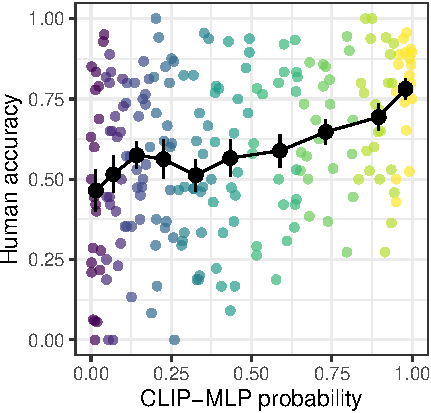
\includegraphics[width=0.7\linewidth]{figs/fig-calibration-1} 

}

\caption[Correlation between human and CLIP-MLP accuracy across deciles of CLIP-MLP accuracy]{Correlation between human and CLIP-MLP accuracy across deciles of CLIP-MLP accuracy. Colored points are individual descriptions, black line is the boostrapped mean and 95\% CI across descriptions for each decile. \label{calibration}}\label{fig:fig-calibration}
\end{figure}
\end{CodeChunk}

TODO methods

pre-reg at \url{https://osf.io/6pv5e}

modeling approach and selection

how well can models proxy humans? are there differences?

tg-matcher 3 (calibration) 61 participants, 64 items each, from a pool
of 217 transcripts spanning the models full accuracy range

\section{Experiment 2}\label{experiment-2}

As a starting point for examining what makes referential expressions
more or less opaque, we had people read the descriptions from the
beginnings and ends and games. Thus, we would be able to check whether
early descriptions (before much partner- or group- specific history
could accumulate, but also before a ``good'' description had been
created) or late descriptions (after both history and practice) would be
easier to understand.

\subsection{Methods}\label{methods}

\subsubsection{Experiment 2a}\label{experiment-2a}

To test our methods and establish a baseline of how well new matchers
could do from reading random transcripts out of order, we ran a 2x2
within subjects design, where we drew the target transcripts from 2 and
6 player games from Experiment 1 of (\textbf{boyce2024?}) and from the
first and last (sixth) blocks of these games. These games had medium
thick communication channels, in that the matchers could send textual
messages to the shared chat interface, but the describer role rotated
each round, and matchers recieved feedback only about whether their
selection was correct or not. We recruited XX participants in May 2024
(check) who each saw 60 trials (15 in each condition). This experiment
was pre-registered at \url{https://osf.io/k45dr}.

\subsubsection{Experiment 2b}\label{experiment-2b}

After observing small condition differences in experiment 2a, we ran a
second study drawing from the more extreme conditions of Experiment 3 in
(\textbf{boyce2024?}). Here, we used a 2x2x2 within subjects design,
drawing our transcripts from the ``thick'' and ``thin'', 2 and 6 person,
1st and last block utterances. The ``thick'' condition had a consistent
describer throughout the entire game, let matchers send messages to the
chat freely, and showed all participants feedback on everyone's
selections, including what the correct answer was. In contrast, the
``thin'' condition, rotated the role of describer, gave feedback only on
individual selections, and describers could not send text messages to
the chat, but could only communicate via 4 emoji buttons (to indicate
level of understanding). Emojis did not have referential content and so
were not included in the transcripts be showed naive matchers. For
experiment 2b, we recruited XX participants in DATE who each saw 64
trials (8 in each condition). This expeirment was pre-registered at
\url{https://osf.io/rdp5k}.

\subsection{Results}\label{results}

Our primary question of interest was how accurate naive matchers would
be at selecting the correct target, and how much this would vary
depending on what game and what round the description came from. We did
not have clear predictions, as we thought there could be countervailing
pressures. On the one hand, the idea of reduction and
partner-specificity would suggest that the conventionalized, later round
utterances would rely on the history of the game that naive matchers
were not privy to, and thus that late round utterances would be more
opaque and difficult to understand. On the other hand, describers gained
practice over repetitions, so later round utterances might better pick
up on visually salient features and include less extraneous verbiage.

In terms of group conditions, based on the patterns of cross-game
similarity in (\textbf{boyce2024?}), we thought that smaller and thicker
games were more likely to rapidly develop ideosyncratic conventions that
would be more opaque than the less ideosyncratic conventions from larger
groups with thinner communication channels.

\begin{CodeChunk}
\begin{figure}[t]

{\centering 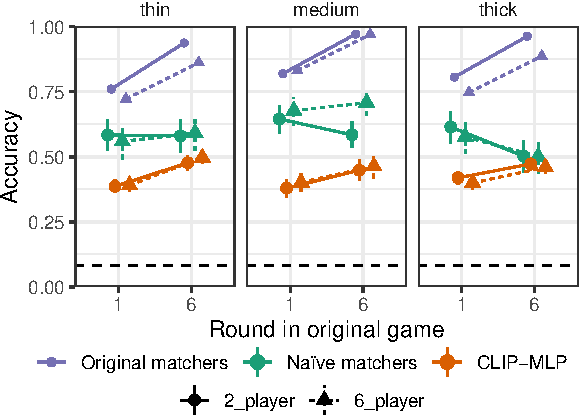
\includegraphics[width=1\linewidth]{figs/fig-condition-1} 

}

\caption[Accuracies for naive humans and the CLIP-MLP model for Experiment 2]{Accuracies for naive humans and the CLIP-MLP model for Experiment 2. Point estimates and 95\% CrI are predictions from the fixed effects of logistic and beta regressions. Bootstrapped mean accuracy from the original matchers is included as a ceiling, and random chance as a baseline. \label{expt2-condition}}\label{fig:fig-condition}
\end{figure}
\end{CodeChunk}

\begin{CodeChunk}
\begin{figure}[t]

{\centering 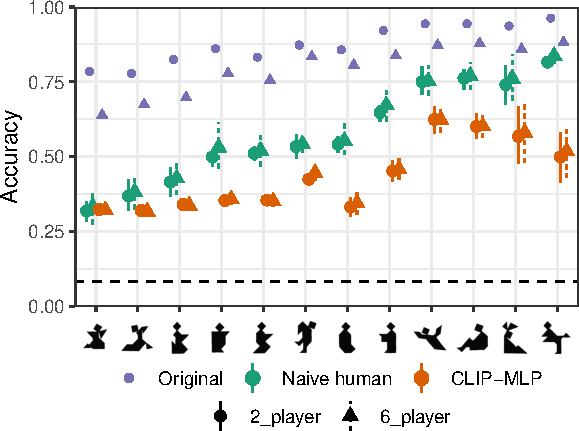
\includegraphics[width=1\linewidth]{figs/fig-2-1} 

}

\caption[Accuracies for naive humans and the CLIP-MLP model for Experiment 2, split out by target image]{Accuracies for naive humans and the CLIP-MLP model for Experiment 2, split out by target image. Point estimates and 95\% CI are predictions from the fixed effects and by-tangram random effects of logistic and beta regressions, bootstrapped across conditions. Bootstrapped mean accuracy from the original matchers is included as a ceiling, and random chance as a baseline. \label{TODO2}}\label{fig:fig-2}
\end{figure}
\end{CodeChunk}

For Experiment 2a, we ran a mixed effects logistic model of naive
matcher accuracy: correct\(\sim\) group\_size \(\times\) round~+
trial\_order~+ (group\_size \(\times\) round\textbar correct\_tangram)~+
(group\_size \(\times\) round~+ trial\_order\textbar workerid). Overall,
naive matchers were above chance (OR: 1.93 {[}1.05, 3.62{]}. There were
not large fixed effects (FIGURE TODO) Last round was slightly lower
accuracy (OR of last round: 0.77 {[}0.53, 1.1{]}). There was not a clear
effect of larger games (OR: 1.15 {[}0.89, 1.47{]}), but round and group
size interacted (OR of 6 player games in round 6: 1.49 {[}1.06, 2.1{]}).
Much of the variation in accuracy was instead driven by the target
images, where the Odds Ratio of the standard deviation of the target was
2.66 {[}1.88, 4.52{]} {[}I'm not sure what the clearest way to present a
stat for this is at all\ldots{]} with some images recieving much more
transparent descriptions than others (FIGURE).

For Experiment 2b we ran a similar mixed effects logistic model:
correct\(\sim\) group\_size \(\times\) thickness \(\times\) round~+
trial\_order~+ (group\_size \(\times\) thickness \(\times\)
round\textbar correct\_tangram)~+ (group\_size \(\times\) thickness
\(\times\) round~+ trial\_order\textbar workerid). Overall, naive
matchers were above chance (OR: 1.81 {[}1.06, 3.08{]}. Again, there was
not a clear pattern of fixed effects. Last round was slightly lower
accuracy (OR of last round: 0.64 {[}0.47, 0.85{]}), but there was an
interaction with thickness, where thin, last round were less opaque (OR:
1.55 {[}1.02, 2.33{]}). TODO do we want to describe some of the other
predictors of this model?

and again some of the uncertainty in estimating the fixed effects was
driven by the strong variation by target image (TODO STATS). 2.25
{[}1.67, 3.59{]}

As additional measures, we also looked whether there was predictive
value from the level of accuracy of the original matchers or the number
of words used by the original describer TODO.

EXPT 1 -- there is a large effect of original accuracy 3.38 {[}2.46,
4.7{]} EXPT 1 -- there is not a substnatial effect of original length
1.05 {[}0.94, 1.17{]}

EXPT 2 -- there is a large effect of original accuracy 2.17 {[}1.7,
2.77{]} EXPT 2 -- there is a slight benefit to longer descriptions 1.1
{[}1.01, 1.2{]}

\subsection{Model results}\label{model-results}

As a computational comparison, we looked at the CLIP-MLP model's
performance on the same descriptions. We used the probability the model
assigned as a measure of the model's accuracy. The CLIP-MLP model was
far above chance, but had lower accuracy than the human participants.

TODO model results

Nothing is significant basically except that thick is better 0.05 {[}0,
0.1{]}.

There is substantial by-tangram variation 0.14 {[}0.09, 0.23{]}

There is an effect of original correct 0.09 {[}0.06, 0.11{]}.

More words is bad for the model -- effect of log words -0.04 {[}-0.05,
-0.03{]}

\section{Yoked v shuffled}\label{yoked-v-shuffled}

TODO methods pre-reg at \url{https://osf.io/zqwp5}

tg-matcher 4 (SPR + yoked/unyoked) 196 participants (99 in yoked, 97 in
shuffled), each saw all 72 trials from 1 of 10 games. games not chosen
at random

\subsection{Human yoked v not yoked
expt}\label{human-yoked-v-not-yoked-expt}

Yoked v shuffled plot of accuracy (+ model?) Human accuracy on yoked v
shuffled presentation (expt 4) (?) no context model comparison on expt 4
dataset?

seeing things in the same order helps look at item level accuracy
differences?

We will exclude individual word RTs that are greater than 2000 ms.

Condition differences: condition refers to yoked or shuffled.

Logistic model of target selection accuracy: Accuracy \textasciitilde{}
original\_rep\_num * condition + viewing\_order + (1 \textbar{} gameId)
+ (1 \textbar{} tangram) + (1 \textbar{} participant)

This dataset was collected using a modified self-paced reading
procedure, but for present purposes, we focus only on the selection
results and not on the incremental reading time patterns.

\begin{CodeChunk}
\begin{figure}[t]

{\centering 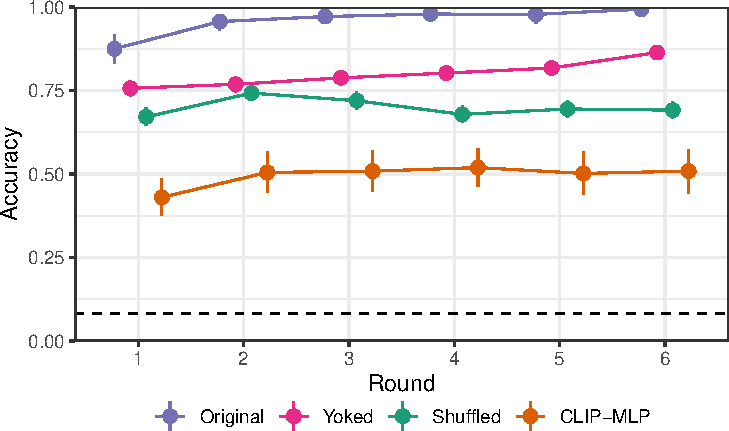
\includegraphics[width=1\linewidth]{figs/fig-yoked-1} 

}

\caption[TODO also TODO add model comparison ?? \label{yoked}]{TODO also TODO add model comparison ?? \label{yoked}}\label{fig:fig-yoked}
\end{figure}
\end{CodeChunk}

not sure how to work model in b/c different scale \ldots{}

\section{Discussion ?}\label{discussion}

\subsection{Part of discussion that Alvin gets to
write??}\label{part-of-discussion-that-alvin-gets-to-write}

Discussion

Understanding varies much more based on item than on anything else;
potentially due to priors or iconicity of image (? that might be beyond
scope -- how well does this match up with say diversity of descriptions)

Models do pretty well? IDK what our model take away is

Especially when there is strong or idiosyncratic reduction, context
helps

role of context

limitations, incuding out of distribution for models

might want to address language comprehension v inference

\section{References}\label{references}

\setlength{\parindent}{-0.1in} 
\setlength{\leftskip}{0.125in}

\noindent

\bibliographystyle{apacite}


\end{document}
